% This file was created by matlab2tikz.
%
%The latest updates can be retrieved from
%  http://www.mathworks.com/matlabcentral/fileexchange/22022-matlab2tikz-matlab2tikz
%where you can also make suggestions and rate matlab2tikz.
%
\documentclass[]{standalone}
\usepackage{amsmath}
\usepackage{graphicx}
\usepackage[pdf]{pstricks}
\usepackage{pgfplots}
\pgfplotsset{compat=newest}
\usepgfplotslibrary{fillbetween}
%% the following commands are needed for some matlab2tikz features
\usetikzlibrary{plotmarks}
\usetikzlibrary{arrows.meta}
\usepgfplotslibrary{patchplots}
\usetikzlibrary{decorations.text}
\usetikzlibrary{shapes.multipart}


\newcommand{\logLogSlopeTriangle}[5]
{
	% #1. Relative offset in x direction.
	% #2. Width in x direction, so xA-xB.
	% #3. Relative offset in y direction.
	% #4. Slope d(y)/d(log10(x)).
	% #5. Plot options.
	
	\pgfplotsextra
	{
		\pgfkeysgetvalue{/pgfplots/xmin}{\xmin}
		\pgfkeysgetvalue{/pgfplots/xmax}{\xmax}
		\pgfkeysgetvalue{/pgfplots/ymin}{\ymin}
		\pgfkeysgetvalue{/pgfplots/ymax}{\ymax}
		
		% Calculate auxilliary quantities, in relative sense.
		\pgfmathsetmacro{\xArel}{#1}
		\pgfmathsetmacro{\yArel}{#3}
		\pgfmathsetmacro{\xBrel}{#1-#2}
		\pgfmathsetmacro{\yBrel}{\yArel}
		\pgfmathsetmacro{\xCrel}{\xArel}
		%\pgfmathsetmacro{\yCrel}{ln(\yC/exp(\ymin))/ln(exp(\ymax)/exp(\ymin))} % REPLACE THIS EXPRESSION WITH AN EXPRESSION INDEPENDENT OF \yC TO PREVENT THE 'DIMENSION TOO LARGE' ERROR.
		
		\pgfmathsetmacro{\lnxB}{\xmin*(1-(#1-#2))+\xmax*(#1-#2)} % in [xmin,xmax].
		\pgfmathsetmacro{\lnxA}{\xmin*(1-#1)+\xmax*#1} % in [xmin,xmax].
		\pgfmathsetmacro{\lnyA}{\ymin*(1-#3)+\ymax*#3} % in [ymin,ymax].
		\pgfmathsetmacro{\lnyC}{\lnyA+#4*(\lnxA-\lnxB)}
		\pgfmathsetmacro{\yCrel}{\lnyC-\ymin)/(\ymax-\ymin)} % THE IMPROVED EXPRESSION WITHOUT 'DIMENSION TOO LARGE' ERROR.
		
		% Define coordinates for \draw. MIND THE 'rel axis cs' as opposed to the 'axis cs'.
		\coordinate (A) at (rel axis cs:\xArel,\yArel);
		\coordinate (B) at (rel axis cs:\xBrel,\yBrel);
		\coordinate (C) at (rel axis cs:\xCrel,\yCrel);
		
		% Draw slope triangle.
		\draw[#5]   (A)-- node[pos=0.5,anchor=north] {1}
		(B)-- 
		(C)-- node[pos=0.5,anchor=west] {#4}
		cycle;
	}
}

\begin{document}
	
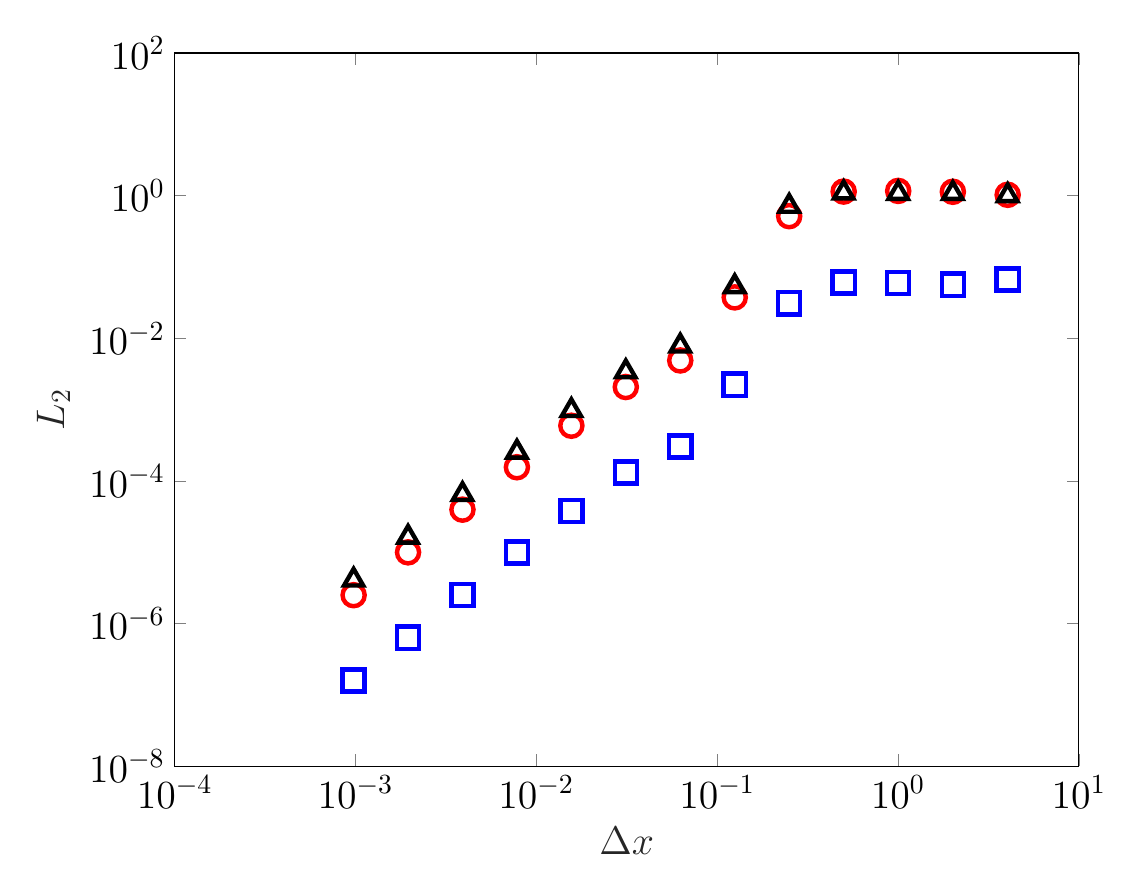
\begin{tikzpicture}
\tikzstyle{every node}=[font=\Large]

\begin{axis}[%
width=4.521in,
height=3.566in,
at={(0.758in,0.481in)},
every axis plot/.append style={ultra thick},
scale only axis,
xmode=log,
xmin=0.0001,
xmax=10,
xtick={0.0001,  0.001,   0.01,    0.1,      1,     10},
xminorticks=false,
xlabel style={font=\color{white!15!black}},
xlabel={\Large $\Delta x$},
ymode=log,
ymin=1e-08,
ymax=100,
ytick={ 1e-08,  1e-06, 0.0001,   0.01,      1,    100},
yminorticks=false,
ylabel style={font=\color{white!15!black}},
ylabel={\Large $L_2$},
axis background/.style={fill=white}
]
 \logLogSlopeTriangle{0.5}{0.2}{0.1}{2}{black};

\addplot [color=blue, draw=none, mark=square, mark size=4pt, mark options={solid, blue}, forget plot]
  table[row sep=crcr]{%
4.04040404040404	0.0667977316044187\\
2.01005025125628	0.0565251008982736\\
1.00250626566416	0.0600244047801842\\
0.500625782227785	0.060369043216863\\
0.250156347717323	0.031027562703989\\
0.125039074710847	0.00223720174663375\\
0.0625097671511174	0.000303213411708855\\
0.0312524415969998	0.00013195585438531\\
0.0156256103754053	3.78678120338089e-05\\
0.00781265259087092	9.90901359842452e-06\\
0.00390628814734519	2.52150220729934e-06\\
0.00195313453678973	6.35217079986901e-07\\
0.000976564884191612	1.59353271500116e-07\\
};
\addplot [color=red, draw=none, mark=o, mark size=4pt, mark options={solid, red}, forget plot]
  table[row sep=crcr]{%
4.04040404040404	1.02894168607817\\
2.01005025125628	1.13471870525711\\
1.00250626566416	1.16651134393852\\
0.500625782227785	1.14209935315627\\
0.250156347717323	0.516295949213657\\
0.125039074710847	0.0375055631709394\\
0.0625097671511174	0.0048956232734942\\
0.0312524415969998	0.00207713643544563\\
0.0156256103754053	0.000595469107815693\\
0.00781265259087092	0.00015580109802979\\
0.00390628814734519	3.96453330936357e-05\\
0.00195313453678973	9.98742874615667e-06\\
0.000976564884191612	2.5054904543415e-06\\
};
\addplot [color=black, draw=none, mark=triangle, mark size=4pt, mark options={solid, black}, forget plot]
  table[row sep=crcr]{%
4.04040404040404	1.00510027333734\\
2.01005025125628	1.07752750295002\\
1.00250626566416	1.07983904140976\\
0.500625782227785	1.09869881739817\\
0.250156347717323	0.712184449316794\\
0.125039074710847	0.05307095900171\\
0.0625097671511174	0.00781225049904385\\
0.0312524415969998	0.00340272133918679\\
0.0156256103754053	0.00097359240010264\\
0.00781265259087092	0.000254452413381455\\
0.00390628814734519	6.47146749585668e-05\\
0.00195313453678973	1.62988208772404e-05\\
0.000976564884191612	4.08829473005837e-06\\
};
%\addplot [color=mycolor1, forget plot]
%  table[row sep=crcr]{%
%4.04040404040404	16.3248648097133\\
%2.01005025125628	4.04030201257544\\
%1.00250626566416	1.0050188126959\\
%0.500625782227785	0.250626173831181\\
%0.250156347717323	0.0625781983032704\\
%0.125039074710847	0.0156347702045448\\
%0.0625097671511174	0.00390747098928691\\
%0.0312524415969998	0.000976715105773881\\
%0.0156256103754053	0.000244159699603973\\
%0.00781265259087092	6.1037540505642e-05\\
%0.00390628814734519	1.52590870900895e-05\\
%0.00195313453678973	3.81473451880083e-06\\
%0.000976564884191612	9.53678973036176e-07\\
%};
\end{axis}
\end{tikzpicture}%
\end{document}